\section{Архитектура библиотеки}

Архитектура библиотеки представлена на рис.~\ref{fig:cubool_architecture}.
Структура библиотеки и ее конечначная функциональность в основном определяется следующими высокоуровневыми требованиями, которые продиктованы как конечными вычислительными задачами на GPGPU, так и наличием существующей инфраструктуры для осуществления экспериментов~\cite{net:cfpq_py_algo}.

\begin{itemize}[noitemsep,topsep=0pt,parsep=0pt,partopsep=0pt]
    \item Поддержка вычислений на Cuda-девайсе.
    \item Поддержка вычислений на CPU.
    \item C-совместимое API для работы с библиотекой.
    \item Python-пакет для работы с примитивами и операциями библиотеки в управляемой высокоуровневой стреде языка Python.
    \item Поддержка логирования, функций для отладки и протопирования конечных пользовательских алгоритмов.
\end{itemize}

\begin{figure}[h]
    \centering
    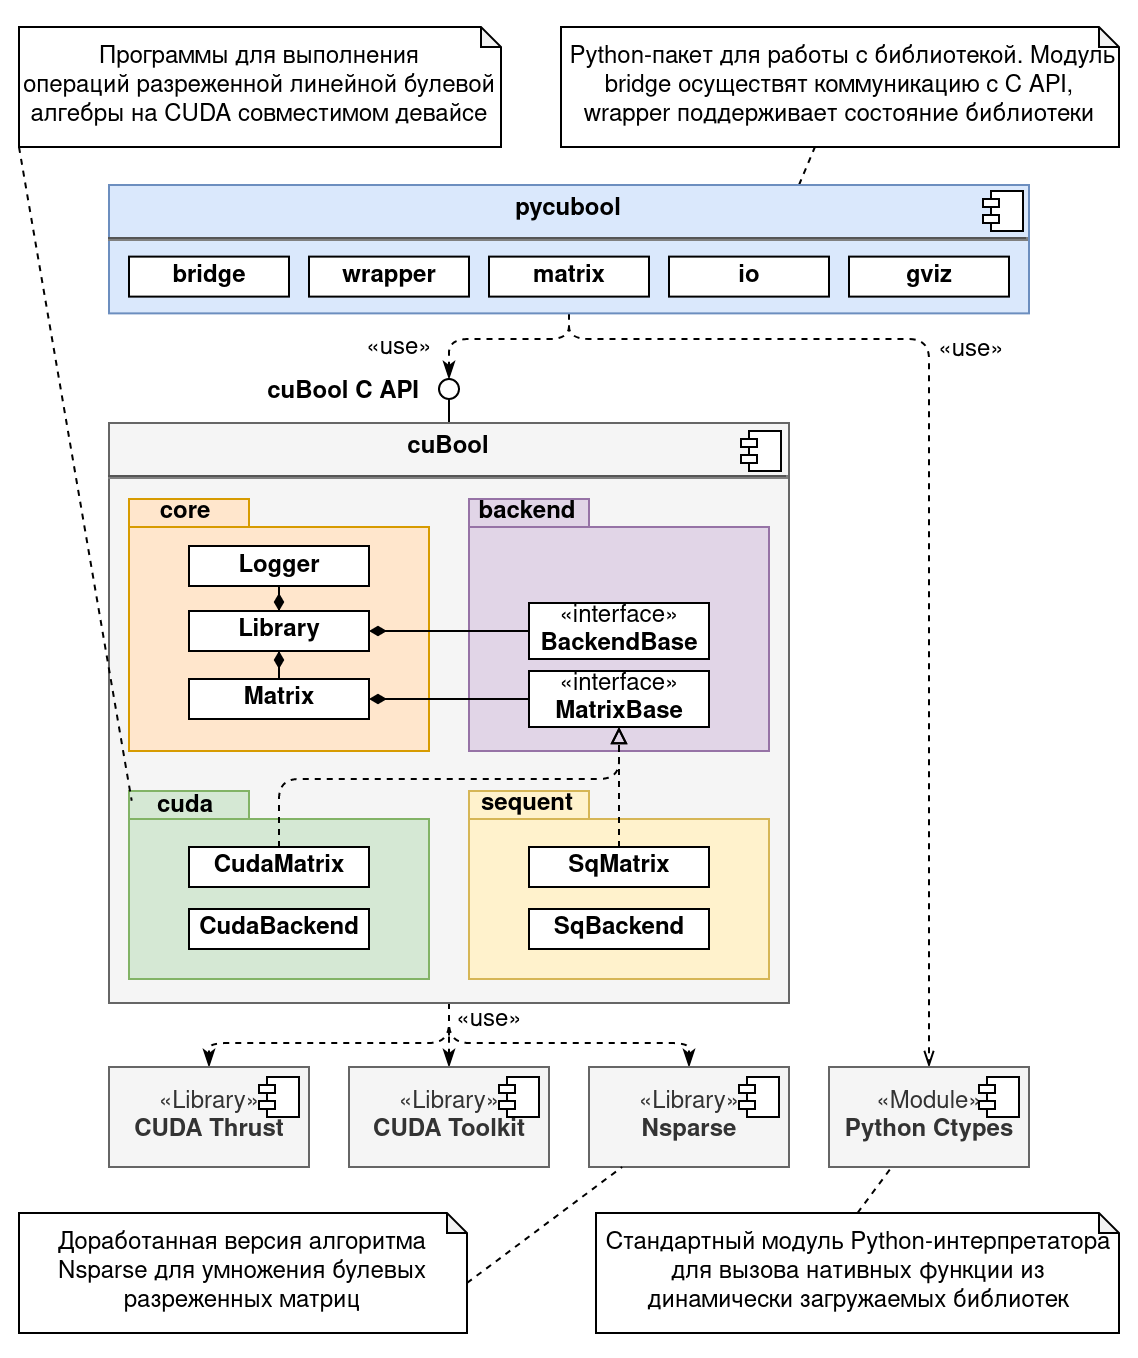
\includegraphics[width=0.8\textwidth]{images/library_architecture.png}
    \caption{Архитектура разработанной библиотеки}
    \label{fig:cubool_architecture}
\end{figure}

\subsection{Компоненты}

\subsubsection*{Core}

Класс \textbf{Library} поддерживает глобальное состояние библиотеки, осуществляет конфигурацию и инициализацию, выбор конкретного вычислительного бэкенда, первичную валидацию вызовов функций и входных данных пользователя, 
а также хранит все созданные пользователем объекты. 

Класс \textbf{Matrix} является proxy-классом, который осуществяет доступ к операциям конкретного вычислительного модуля, выбранного пользователем на этапе инициализации всей библиотеки.
Данный подход позволяет не только динамически выбирать платформу вычислений, 
но и позволяет осуществлять дополнительную обработку ошибок, 
а также поддерживать дополнительные операции над матрицами.

Класс \textbf{Logger} осуществляет логгирование в выбранный пользователем текстовый файл в процессе использования функций библиотеки, а также позволяет профилировать операций и также сохранять время их выполенения в текстовом виде.

\subsubsection*{Backend}

Интерфейс \textbf{MatrixBase} предоставляет набор основных функций и операций, которые каждый вычислительный модуль должен реализовывать, чтобы предоставляемые им матрицы можно было использовать в \textbf{Core} непосредственно для вычислений.

Интерфейс \textbf{BackendBase} описывает базовый контракт, которой должен предоставлять вычислительный модуль. Данный интерфейс включает в себя функции для создания и удаления матриц, спефичных для этого модуля, а также функции для корректной инициализации, поддержания глобального состояния и завершения работы.

\subsubsection*{Cuda}

Класс \textbf{CudaMatrix} предоставляет реализацию матрицы и операций для осуществления вычислений на Cuda-девайсе. \textbf{CudaMatrix} хранит структуру и данные матрицы (ненулевые элементы) в видео-памяти и использует Nvidia GPU для вычислений.

Данный вычислительный модуль выбирается по умолчанию, если в компьтере пользователся имеется Cuda-девайс.
Однако пользователь всегда может выбрать \textbf{Sequential} вычисления, если это требуется. 

\subsubsection*{Sequential}

Предоставляет реализацию класса матрицы и операций над ней для вычислений на CPU. Все вычислений осуществляются последовательно, в однопоточном режиме, что не требует дополнительных библиотек или компонентов.

Данных вычислительный модуль используется по умолчанию на устройствах без Cuda-девайса. 
Данный подход позволяет использовать библиотеку всем пользователям без исключения. 
Также данный подход может быть удобен для прототипирования алгоритмов на локальном компьютере, 
чтобы позже запустить вычисления на высокопроизводительном сервере с поддержкой Cuda.

\subsubsection*{Pycubool}

Python-пакет предоставляет доступ к примитивам и операциям библиотеки в языковой среде Python.
Модуль \textbf{matrix} предоставляет доступ к классу матрицы и основным операциям, дотсупным в C API.
Модуль \textbf{bridge} осуществляет коммуникацию с библиотекой через механизмы вызова нативных методов. 
Модуль \textbf{wrapper} поддерживает глобальное состояние библиотеки во время работы Python-интерпретатора. 
Модули \textbf{io} и \textbf{gviz} предоставляют доступ к операциям ввода/вывода данных, 
позволяют загружать или сохранять матрциы в текстовом формате, 
а также экспортировать набор матриц в виде графа в формате GraphViz, 
что может быть полезно для отладки пользовательских алгоритмов.

\subsection{Последовательнось обработки операций}

На рис.~\ref{fig:cubool_sequence} представлена последовательность обработки вычислительной операции над матрицей на Cuda-девайсе.

Пользовательский Python-код инициирует выполнение операции над мамтрицей или несколькими матрицами.
Этот вызов обрабатывает пакет \textbf{pycubool}, который осуществляет первичную базовую валидацию аргументов, запаковывает их и передает в нативную функцию \textbf{cuBool C API}.
На стороне реализации данного интерфейса полученные аргументы приводятся к требуемому типу и передаются далее в модуль \textbf{Core}, 
который поддерживает состояние библиотеки, 
осуществяет валидацию аргументов, а также определяет допустимость выполнения операции. 
Далее вызов передается непосредственно вычислительному модулю \textbf{Cuda}, 
который осуществляет подготовку и непосредственный запуск вычислений на сороне \textbf{Nvidia GPU}. 

Когда вычисления завершаются, \textbf{Cuda}-модуль обновляет состояние матриц в соответсвии с полученными результами. 
Модуль \textbf{Core} осуществяет финальное логирование операции, 
а также сохраняет временные показатели выполнения вычислений в файл (опционально), 
и возвращает в качестве результата выполнения статус операции или возможное исключение, 
которое могло возникнуть на этапе выполнения операции. 
\textbf{cuBool C API} осуществяет финальную обработку исключения (если таковое возникло), 
и возвращет вызываещему числовой идентефикатор статуса операции. 

В результате выполнения операции \textbf{pucubool} уведомляет пользователя о потенциально возникших ошибках и возвращает управление из вызываемой функции. 
Обновленное состояние библиотеки находится в \textbf{Core}, а состояние матриц после выполнения операций хранится на стороне \textbf{Cuda}-модуля. 

\begin{figure}[]
    \centering
    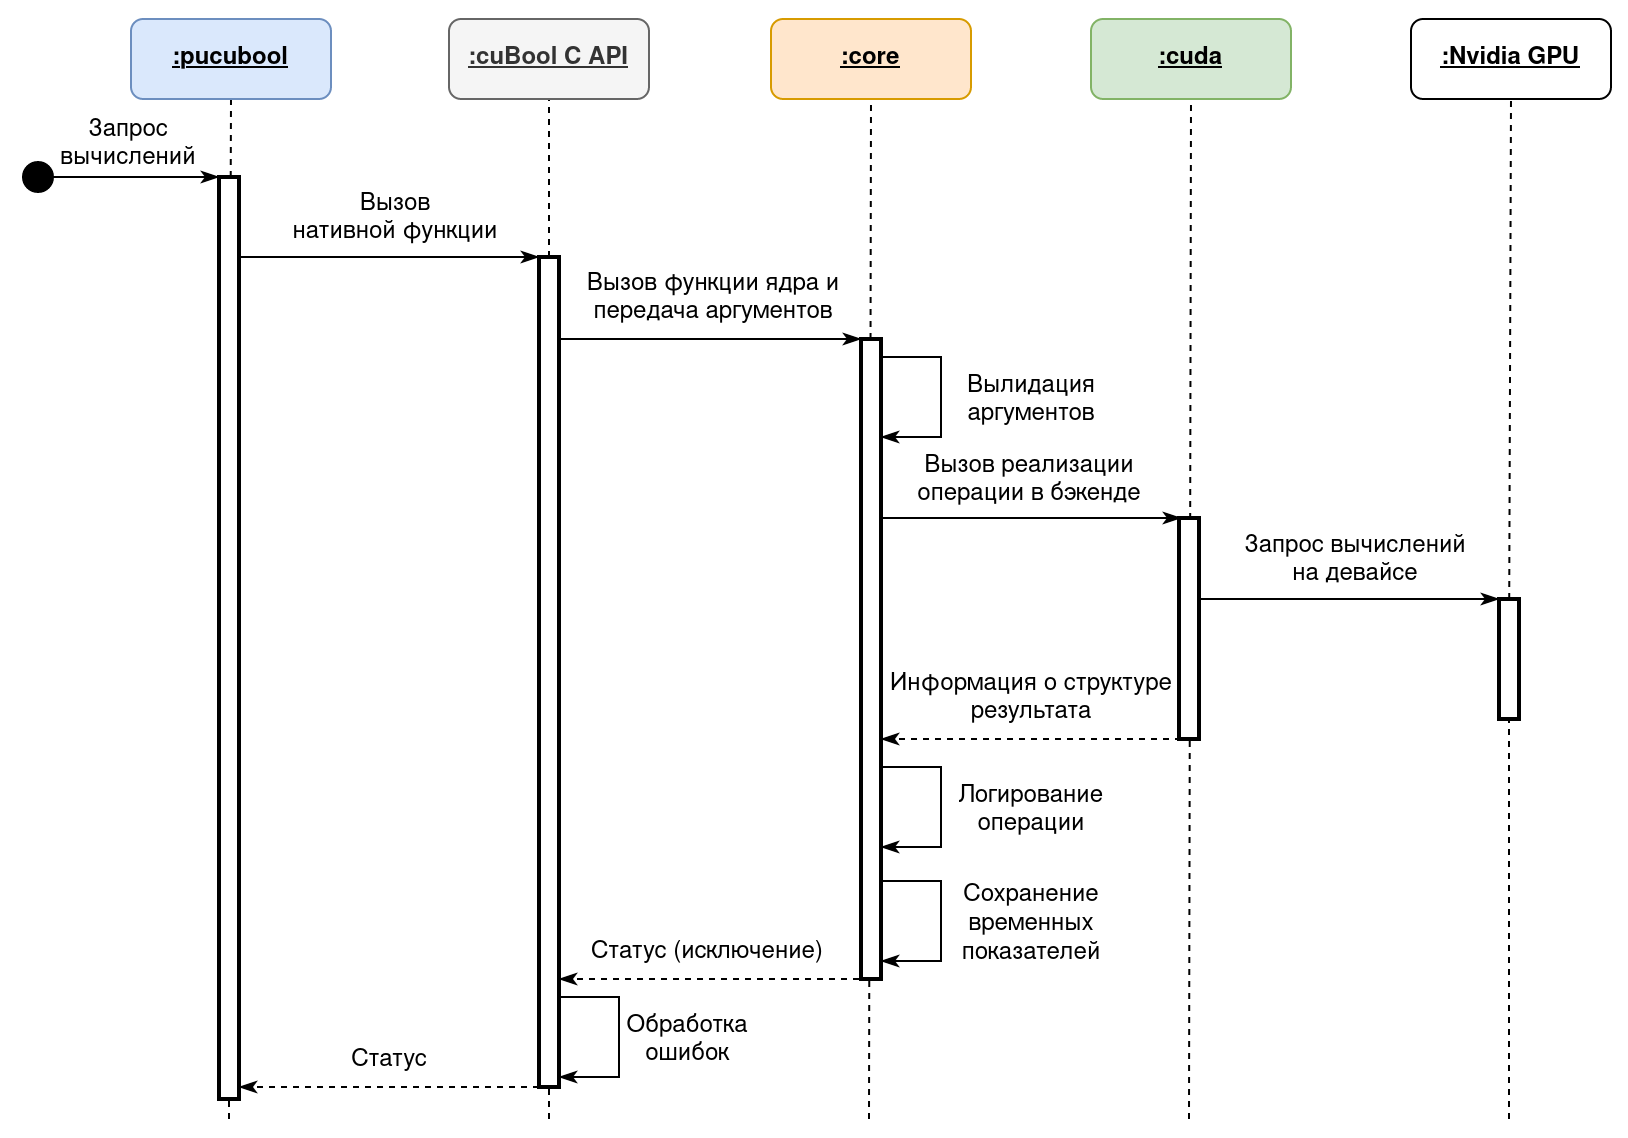
\includegraphics[width=0.9\textwidth]{images/library_sequence_use.png}
    \caption{Последовательность выполнения вычислительной матричной операции на Nvidia GPU с использованием pycubool}
    \label{fig:cubool_sequence}
\end{figure}
